\chapter{Results and Discussion}
\section{Analisi parametri utilizzati}
\begin{figure}[H]
	\centering
	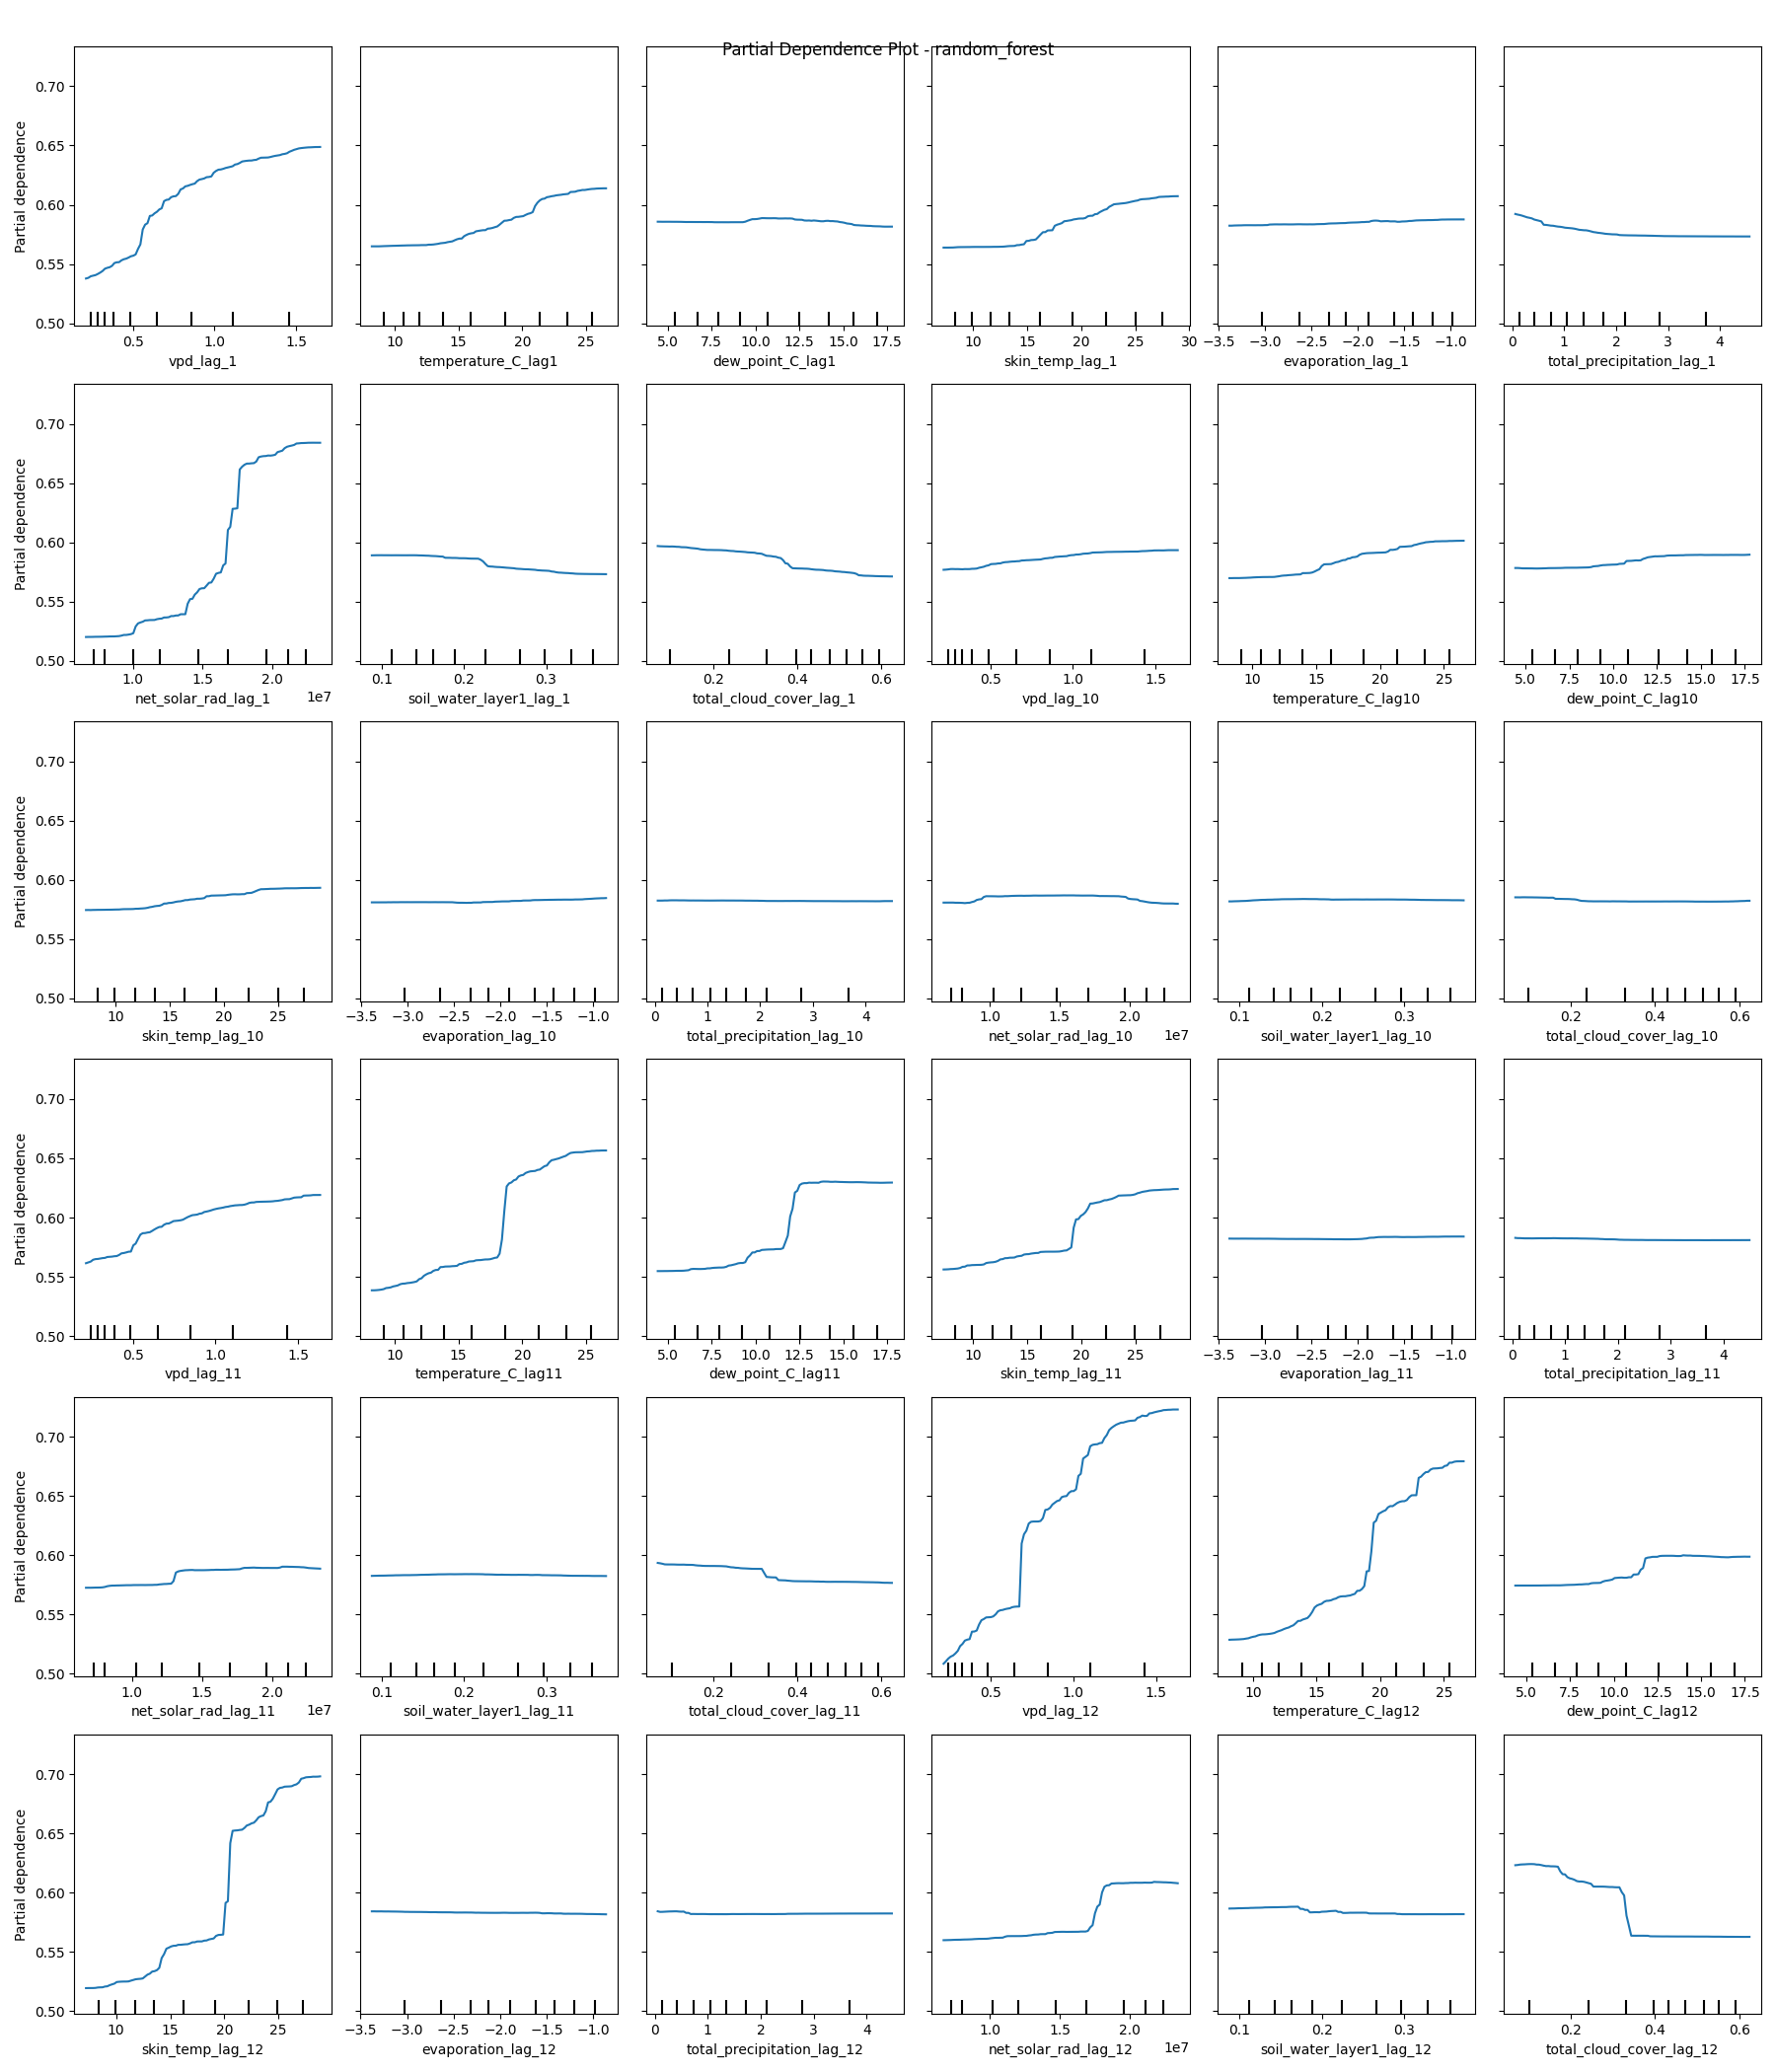
\includegraphics[width=0.8\textwidth]{images/pdp_group_random_forest_v2}
	\caption{Partial Dependence Plot Random Forest}
	\label{fig:PartialDependence_RF}
\end{figure}
Questi partial dependence plot prendono come caso d'esempio il modello del Random Forest per mostrare come al variare dei vari parametri usati come input per i modelli analizzati varino le previsioni effettuate dallo stesso. Sull'asse X si trovano i valori presi dal parametro, mentre sull'asse y il VPD predetto, se la curva relativa al parametro sale vuol dire che all'aumentare del parametro aumenta il valore predetto, se la curva scende, scende anche il valore predetto, mentre ancora se la curva tende ad essere stabile o quasi parallela all'asse X vuol dire che il parametro ha un'influenza trascurabile nella previsione.
\section{Analisi metriche risultanti}
Come esplicitato la comparazione tra i vari modelli testati è stata eseguita attraverso l'analisi delle 5 metriche risultanti per ciascun modello. Queste metriche come già anticipato sono:
\begin{itemize}
	\item il coefficiente di correlazione (CC) per comprendere la capacità del modello di seguire, con le sue predizioni, lo stesso andamento dei valori reali
	\item MAE e RMSE per capire l'errore assoluto medio dei valori predetti dal modello rispetto a quelli reali, con la differenza che l'RMSE aumenta l'impatto di un errore se la previsione è molto lontana dal valore reale
	\item RAE e RRSE seguono lo stesso principio dell' MAE e del RMSE con la differenza che l'errore non è assoluto ma relativo alla previsione che un modello basato solo sulla media dei valori in input fornirebbe
\end{itemize}
L'analisi di queste metriche mostra come i modelli dai risultati più solidi e costanti siano Additive Regression e Random Forest, non perchè abbiano i valori migliori per ogni singola metrica ma perchè in entrambi i tipi di split e per tutte le metriche si attestano sempre tra i migliori modelli utilizzati, particolare è il caso del linear regression che ha buoni risultati soprattutto con RMSE e l'RRSE, ciò dovrebbe significare che anche se in media esso sbagli leggermente di più di Random Forest ed Additive Regression, i suoi errori in media sono leggermente meno grandi, un'altra costante nelle analisi è che il modello REPTree si attesta costantemente come il peggiore tra quelli utilizzati, caso più particolare è invece quello delle reti neurali, le quali sono costantemente tra i modelli migliori per quanto riguarda il coefficente di correlazione e gli errori relativi, al contrario però dimostrano dei valori di errore medio assoluto più alti rispetto alle controparti che eseguono algoritmi di machine learning più tradizionali. Un altro fenomeno da evidenziare è come tendenzialmente i risultati sono migliori quando il dataset utilizzato è quello che esegue lo split unicamente per province ignorando l'arco temporale dei dati, con solo due eccezioni ovvero l'errore relativo medio del Linear Regression e dell'Additive Regression che migliora con lo split temporale.\\
\begin{figure}[H]
	\centering
	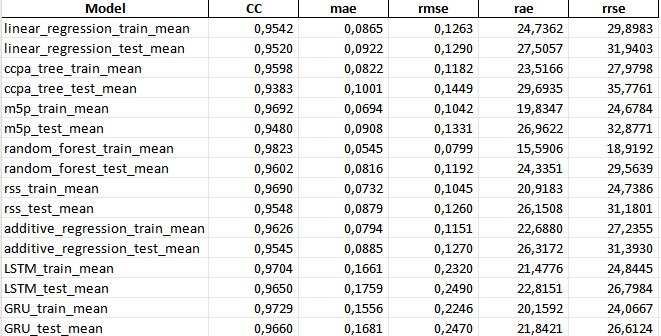
\includegraphics[width=0.8\textwidth]{images/Cross_values}
	\caption{Tabbella contenente tutti i risultati dei modelli con input dataset sottoposto unicamente a split-spaziale}
	\label{fig:Cross_values}
\end{figure}
\begin{figure}[H]
	\centering
	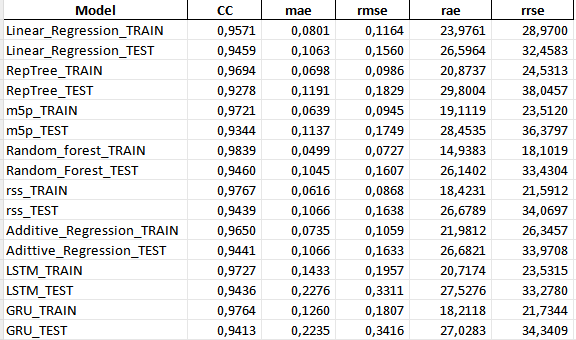
\includegraphics[width=0.8\textwidth]{images/8020_values}
	\caption{Tabbella contenente tutti i risultati dei modelli con input dataset sottoposto unicamente a split-temporale}
	\label{fig:8020_values}
\end{figure}
\section{Rappresentazioni grafiche}
\subsection{Machine learning tradizionale}
Per visualizzare graficamente le metriche mostrate sono stati stampati gli scatter-plot relativi al test set, i grafici hanno sull'asse X il valore di vpd reale del test set mentre sull'asse y quello predetto, di conseguenza i punti presenti sono le singole osservazioni nel test set, esse mostrano per esempio che la maggior parte dei valori del vpd si concentrano in valori molto bassi con una densità sempre minore più ci si sposta nella parte destra e alta dei grafici, ciò è coerente con la realtà dei dati, perchè i valori alti si riscontrano per la maggior parte solo nei mesi estivi, infine le due rette rappresentano, una (quella rossa) la retta creata da tutti i valori reali di vpd, mentre l'altra rappresenta la retta di regressione calcolata sui punti effettivi predetti in funzione di quelli reali.\\
\begin{figure}[H]
	\centering
	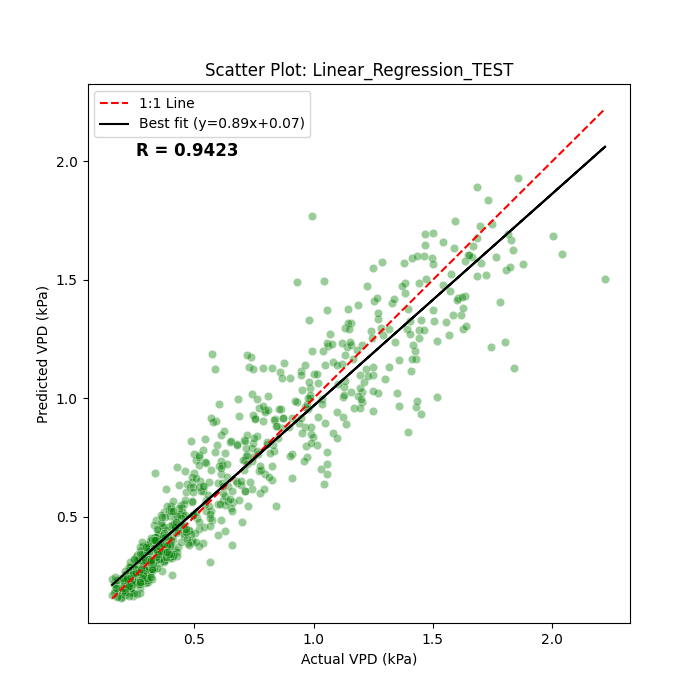
\includegraphics[width=0.45\textwidth]{images/8020_Linear_Regression_TEST}
	\caption{Scatter plot delle previsioni rispetto ai valori reali di VPD sul dataset con split temporale per Linear Regression, la retta di best fit mostra una leggera sottostima per valori di VPD più elevati}
	\label{fig:Linear_Regression_plot}
\end{figure}
\begin{figure}[H]
	\centering
	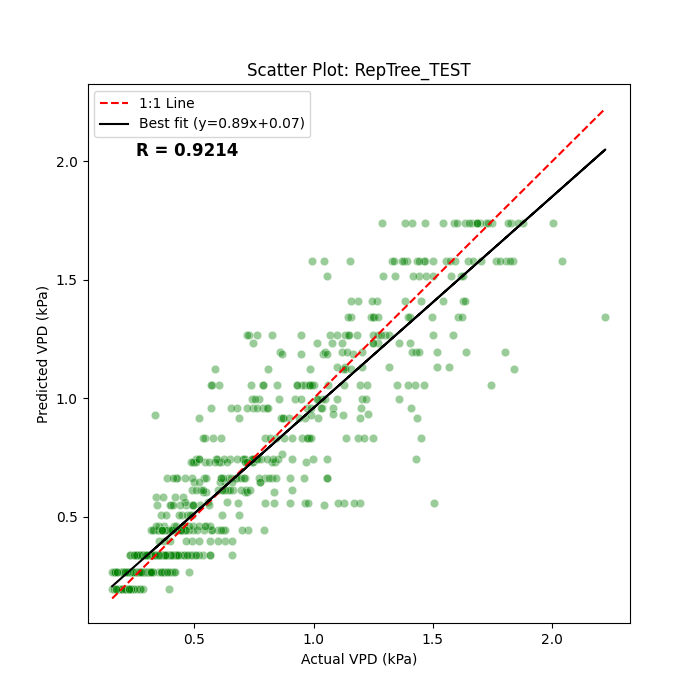
\includegraphics[width=0.45\textwidth]{images/8020_RepTree_TEST}
	\caption{Scatter plot delle previsioni rispetto ai valori reali di VPD sul dataset con split temporale per REPTree, il pattern è dovuto alla natura discreta delle previsioni create dalle foglie dell'unico albero}
	\label{fig:RepTree_plot}
\end{figure}
\begin{figure}[H]
	\centering
	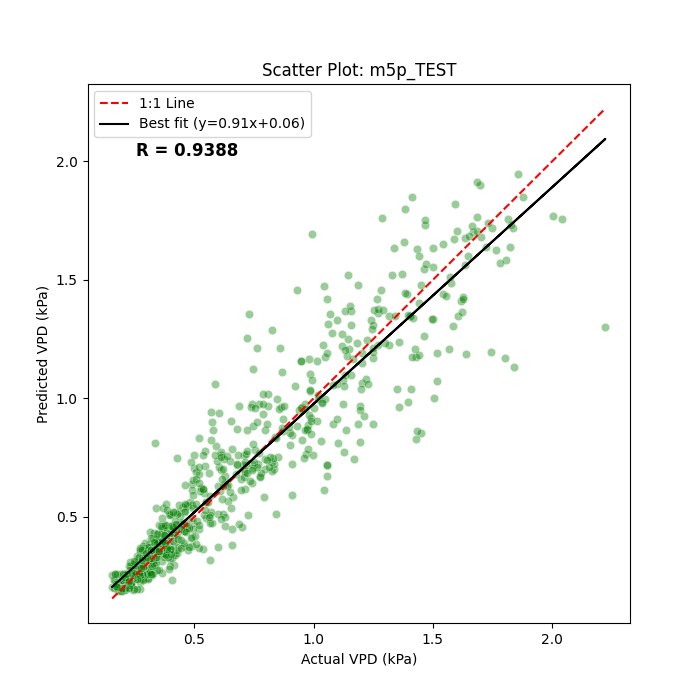
\includegraphics[width=0.45\textwidth]{images/8020_m5p_TEST}
	\caption{Scatter plot delle previsioni rispetto ai valori reali di VPD sul dataset con split temporale per M5P}
	\label{fig:M5P_plot}
\end{figure}
\begin{figure}[H]
	\centering
	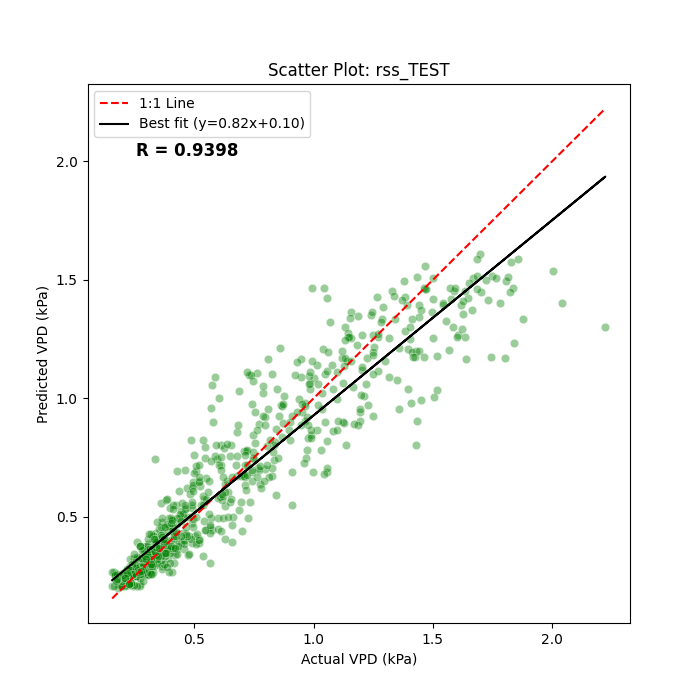
\includegraphics[width=0.45\textwidth]{images/8020_rss_TEST}
	\caption{Scatter plot delle previsioni rispetto ai valori reali di VPD sul dataset con split temporale per Random Subspace, mostra il maggior effetto di compressione verso la media delle previsioni}
	\label{fig:RSS_plot}
\end{figure}
\begin{figure}[H]
	\centering
	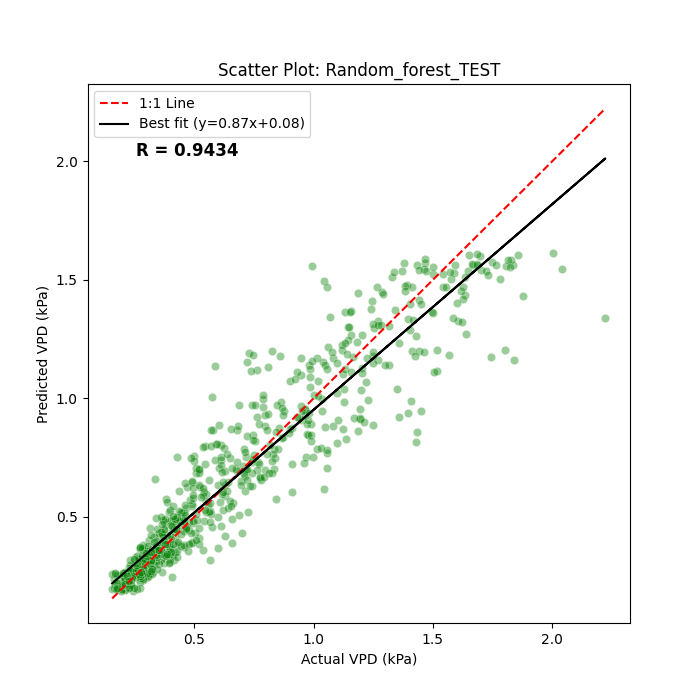
\includegraphics[width=0.45\textwidth]{images/8020_Random_forest_TEST}
	\caption{Scatter plot delle previsioni rispetto ai valori reali di VPD sul dataset con split temporale per Random Forest, mostra una leggera sottostima dei valori di VPD più estremi}
	\label{fig:Random_Forest_plot}
\end{figure}
\begin{figure}[H]
	\centering
	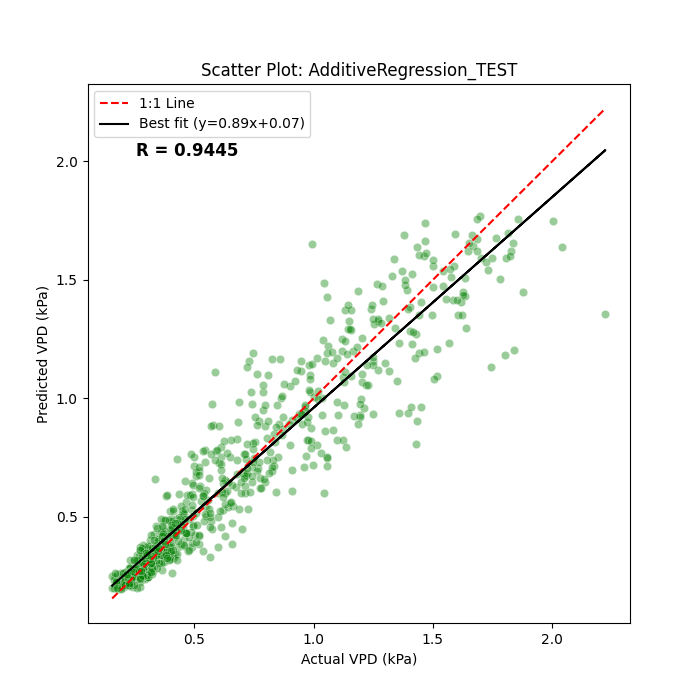
\includegraphics[width=0.45\textwidth]{images/8020_AdditiveRegression_TEST}
	\caption{Scatter plot delle previsioni rispetto ai valori reali di VPD sul dataset con split temporale per Additive Regression, mostra una distribuzione dei residui relativamente omogenea}
	\label{fig:Additive_Regression_plot}
\end{figure}
\subsection{LSTM e GRU}
Per quanto riguarda le reti LSTM e GRU sono stati analizzati gli andamenti della funzione di loss dell'errore quadratico medio. I grafici riportano sull'asse X il numero di epoche mentre sull'asse Y il valore della funzione di loss, le due curve invece vengono calcolate su due sottoinsiemi di dati differenti, la blu sui dati di training e l'arancione su un validation set.\\
\begin{figure}[H]
	\centering
	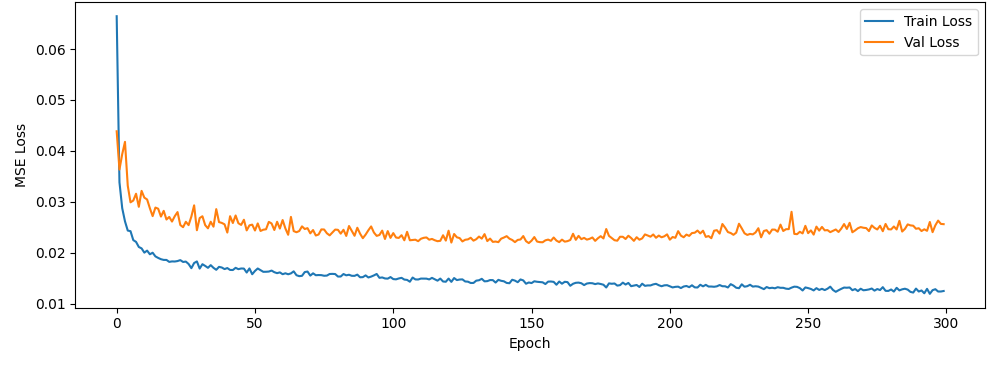
\includegraphics[width=0.45\textwidth]{images/loss_lstm}
	\caption{Andamento della funzione di loss nell'addstramento del modello LSTM, mostra come la curva relativa al validation set si stabilizzi dopo le prime epoche suggerendo una riduzione delle epoche}
	\label{fig:LSTM_loss}
\end{figure}
\begin{figure}[H]
	\centering
	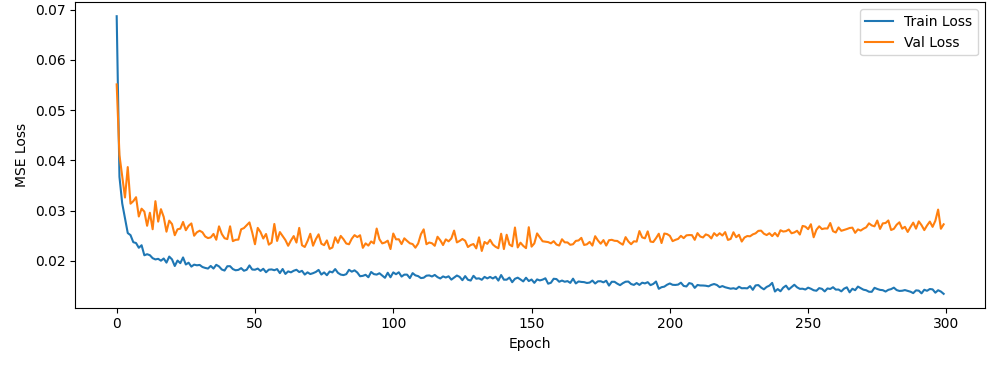
\includegraphics[width=0.45\textwidth]{images/loss_gru}
	\caption{Andamento della funzione di loss nell'addestramento del modello GRU, mostra come la curva relativa al validation set si stabilizzi dopo le prime epoche suggerendo una riduzione delle epoche}
	\label{fig:GRU_loss}
\end{figure}
\section{Discussione dei risultati}
Questo studio ha come obiettivo quello di valutare le prestazioni di 8 algoritmi di apprendimento automatico, ovvero, Linear Regression, RepTree, M5P, Additive Regression, Random Forest, Random Subspace, LSTM e GRU, per quanto riguarda la loro capacità di previsione a lungo termine per i valori di VPD nelle province siciliane.
Attraverso la funzione PACF sono stati rivelati i mesi i cui valori hanno una maggiore influenza sui vpd futuri, essi si sono rivelati i lag 1, 10, 11 e 12, fatto ciò sono stati selezionati i parametri da utilizzare come input per i modelli da valutare essi sono stati i vpd, la temperatura, la temperatura di rugiada, la temperatura del suolo, evaporazione totale, le precipitazioni totali, la radiazione solare, l'umidità del suolo e la copertura totale delle nuvole tutti relativi ai lag selezionati precedentemente, tuttavia i partial dependence plot hanno dimostrato come solo una frazione di questi parametri abbia un effetto reale sulle predizioni effettuate dai vari modelli, dimostrando probabilmente come ci sia una ridondanza di informazioni tra i vari parametri usati o più semplicemente come alcuni di essi non abbiano una correlazione col vpd.\\
I risultati mostrano come tutti i modelli forniscano dei risultati accettabili per quanto riguarda l'accuratezza delle previsioni, un'analisi comparativa più specifica però mostra come i modelli dell'Additive Regression e del Random Forest si attestino come quelli più stabili, sia per quanto riguarda lo split temporale che quello spaziale, altre due considerazioni di carattere generale tra i vari modelli testati sono innanzitutto che il REPTree si attesta constantemente come il peggiore tra tutti, probabilmente perchè essendo costituito da un unico albero le foglie si adattano troppo unicamente ai dati di training non riuscendo a generalizzare per valori di test mai visti, l'altra considerazione da fare riguarda i modelli LSTM e GRU i quali riescono a generalizzare e comprendere bene il trend dei valori del VPD ma hanno sistematicamente errori assoluti medi maggiori rispetto agli altri modelli, ciò potrebbe essere causato dal processo di normalizzazione oppure dal fatto che in modelli di reti neurali ricorrenti forniscono prestazioni migliori quando i lag temporali forniti in input sono continui e non selezionati a priori in base alla loro influenza diretta sul valore da predire, ciò potrebbe suggerire sviluppi in lavori futuri incentrati unicamente su questi tipi di algoritmi, per verificare tale ipotesi.\\
Un'altra costatazione da fare riguarda i due tipi di split utilizzati, i risultati ottenuti mostrano come sistematicamente i modelli testati abbiano nella maggior parte dei casi prestazioni leggermente migliori quando lo split è eseguito unicamente a livello spaziale, ciò potrebbe suggerire come le differenze in termini di vpd tra le varie province non siano così grandi da portare un modello che si è allenato unicamente su altre province siciliane a non effettuare previsioni abbastanza accurate, l'effetto che dati mai visti avrebbe dovuto creare potrebbe esser stato ancora più attenuato dal fatto che, essendo i dati sia del train che del test riferiti allo stesso arco temporale, i modelli potrebbero essersi adattati ai trend riscontrati nelle province di test già allenandosi nelle province di training.

\label{sec:results}